\begin{enumerate}[(a)]
\item Sketch the root locus corresponding to the possible closed loop pole locations for the following feedback system
\begin{center}
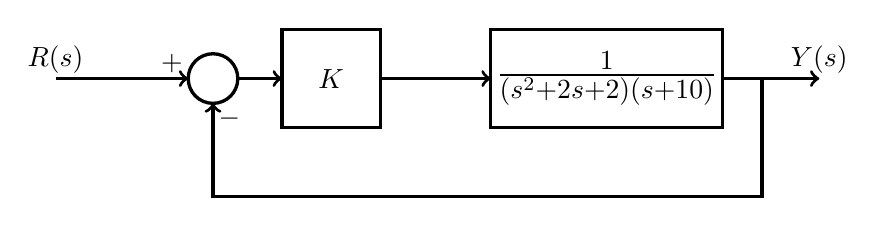
\begin{tikzpicture}[scale=1,inner sep=0pt,outer sep=0pt,very thick,
sysblock/.style={draw,rectangle,inner sep=2pt,minimum width=1.25cm,minimum height=1.25cm,very thick}]
\draw (2,0) node[draw,circle] (sum1) {$\rule{0pt}{18pt}$};
\draw (3.5,0) node[sysblock] (Kp) {$ K$};
\draw (7,0) node[sysblock] (G) {\Large $\frac{1}{(s^2+2s+2)(s+10)}$};
\draw[->] (0,0) node[above=2pt] {$R(s)$} -- (sum1.180) node[above left=2pt] {$+$};
\draw[->] (sum1.0) --  (Kp);
\draw[->] (Kp) -- (G);
\draw[->] (G) -- ++(2.7,0) node[above=2pt] {$Y(s)$};
\draw[->] (G.0) ++(.5,0) -- ++(0,-1.5) -| (sum1.-90) node[below right=2pt] {$-$};
\end{tikzpicture}
\end{center}
%\vspace{3in}
\item Suppose the feedback control system is modified to be the following. Calculate the value of $a$ such that two of the closed loop poles asymptotically approach a line with real part ${\rm Re}\{s\}=-2$ as $K\rightarrow \infty$.
\begin{center}
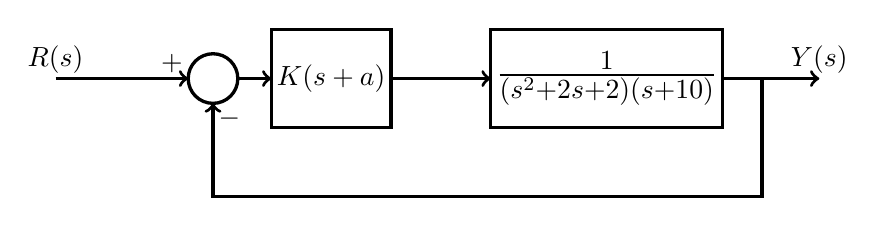
\begin{tikzpicture}[scale=1,inner sep=0pt,outer sep=0pt,very thick,
sysblock/.style={draw,rectangle,inner sep=2pt,minimum width=1.25cm,minimum height=1.25cm,very thick}]
\draw (2,0) node[draw,circle] (sum1) {$\rule{0pt}{18pt}$};
\draw (3.5,0) node[sysblock] (Kp) {$ K(s+a)$};
\draw (7,0) node[sysblock] (G) {\Large $\frac{1}{(s^2+2s+2)(s+10)}$};
\draw[->] (0,0) node[above=2pt] {$R(s)$} -- (sum1.180) node[above left=2pt] {$+$};
\draw[->] (sum1.0) --  (Kp);
\draw[->] (Kp) -- (G);
\draw[->] (G) -- ++(2.7,0) node[above=2pt] {$Y(s)$};
\draw[->] (G.0) ++(.5,0) -- ++(0,-1.5) -| (sum1.-90) node[below right=2pt] {$-$};
\end{tikzpicture}
\end{center}\end{enumerate}